\section{Access Methods}


\subsection{Introduction}

We are now looking at layer 3 and 4 in Figure \ref{fig:arch}. We know now how data is brought from storage to memory - in this section we focus on how it is represented and organized in memory (how tuples are arranged within blocks and indexes), which impacts processing speed and hardware features that can be used.

\paragraph{Workload}
A DB system and its access methods can be constructed to handle a certain kind of workload (on-line transaction / analytic processing = OLT/AP). The type of workload also influences the choice of hardware. We have:
\begin{itemize}
    \item \textbf{Transactional (OLTP):} Workload is dominated by (large amount of) short transactions with updates and modifications (high I/O), usually point queries (targeting one tuple), sensitive to contention, needs lots of processing power. Fits the traditional design of a relational engine.
    \item \textbf{Analytical (OLAP):} Workload is dominated by complex queries combining many tables, usually only read queries, needs large amount of memory and processing power. Usually uses a data warehouse system.
\end{itemize}

\paragraph{Trade-Offs}
Trade-offs made in a DB design can include:
\begin{itemize}
    \item More compact representations vs. more complex processing.
    \item More indexes vs. more space and less maintenance cost.
    \item Row store for OLTP vs. column store for OLAP.
    \item The amount of unused space to keep for updates / movements.
    \item etc.
\end{itemize}


\subsection{Physical Storage Organization}


\paragraph{Finding a Block}
Each segment has a segment header which contains a (linked) list of used and free blocks. Both lists keep track of block IDs (Extent, Offset) while the free list also keeps track of the available space. This system is a potential bottleneck, especially for modification transactions.

\textbf{Improving Performance:} Using several free lists for faster concurrent transactions, making the traversal of the free list fast (sorting by size, keep it short, etc.), efficient search for holes in all blocks, etc.

\paragraph{Finding a Tuple / Record}
Each block, next to a block header, maintains a list of pointers (offsets) to all the slots in it that store a tuple each. Each tuple has an ID (Block ID, Offset). The slots / tuples are not uniform in size (hence the offsets).

\textbf{Changes:} Too large for the slot - keep a new pointer in original position to new location of tuple (can be in a different block, ID stays the same). Deletion - remove pointer. Smaller - just leave space empty. Insertion - use a block with enough free space (compact it if needed).

\paragraph{Tuple / Record Structure}
A tuple contains a header (validity flags for deletion, visibility info for concurrency control, bit map of null values, etc.) and attributes (data / pointer to data for each non-null attribute) as seen in Figure \ref{fig:tuple}. A relational DB does \textbf{not} store schema information (table name, data types of attributes, number of attributes, etc.) in a tuple - this is in contrast to schema-less systems (see later).

\begin{figure}[h]
	\centering
	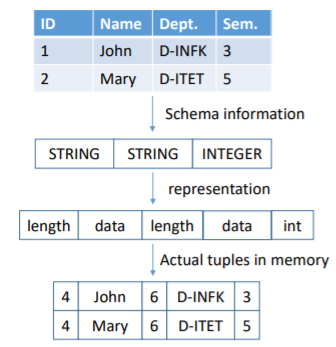
\includegraphics[scale=0.6]{images/2-tuple.PNG}
	\caption{Tuple representation in memory (header omitted - usually in front of data).}
	\label{fig:tuple}
\end{figure}

\paragraph{Record Layout Optimizations}
The serial representation as seen in Figure \ref{fig:tuple} is intuitive but has a linear time to access each attribute. To improve the access time, we can either have a fixed sized part at the beginning of a tuple that stores offsets instead of lengths with each pointer pointing to the tail of an attribute (constant access time for each attribute or simply reorder the attributes such that variable length data (e.g. strings) is placed at the end (again with the pointer system from above). %TODO: how is this constant access if we first have to find out which offset we need?

\paragraph{Data Types}
\begin{itemize}
    \item \textbf{Integer Numbers:} %TODO how representation, similar to C
    \item \textbf{Real Numbers:} IEEE-754 standard for variable precision or fixed point representations for fixed precision (avoids rounding errors). %TODO
    \item \textbf{Strings and BLOBS (Binary Large Objects):} Length and data.
    \item \textbf{Time, Coordinates, Points, etc.:} System specific.
\end{itemize}

When a tuple / single attribute is very big (usually in reference to block size), instead of storing the whole thing one can store the fixed part of it and a pointer to the variable part (potentially in a different block or even a DB-external file). Since it is common that those attributes are not processed by queries, putting them somewhere else speeds up scanning operations. This is usually the case for BLOBS (e.g. pictures, text, etc.).

\paragraph{Row Store}
Tuples are stored as described so far with all the attributes staying together (just as seen as in a table). Allows for quick access and retrieval of an entire tuple. Is usually used in OLTP systems where operations are mostly carried out on individual tuples. When only retrieving a single attribute, a lot of unnecessary data is scanned and brought into the cache since we carry entire blocks.

\paragraph{Column Store}
The data is stored by columns, i.e. each block contains columns instead of rows of a table. Usually used on OLAP / in-memory DBs. Each column either has virtual IDs (order = ID, as in row store, safes space) or explicit IDs which are repeated for each column s.t. each column can be treated individually and (relative) order does not matter. Uses the cache very efficiently. Easy to compress. Improves bandwidth. Disadvantages: When an entire tuple is needed, we need to access several blocks. Complex if a tuple needs to be reconstructed as an intermediate / final result. Modifications are more difficult.

\textbf{Vectorized Processing / SIMD:} Simultaneously performing an operation on a vector of values. Column store is the perfect data representation for this. Very useful for numeric values and bit comparisons.

\paragraph{Partition Attributes Across (PAX)}
An alternative tuple representation as seen in Figure \ref{fig:pax}. A block is divided into mini-blocks and contains several tuples but is organized as a column store. Reconstructing the tuple does not require access to several blocks. See papers (below) for more info.

\begin{figure}[h]
	\centering
	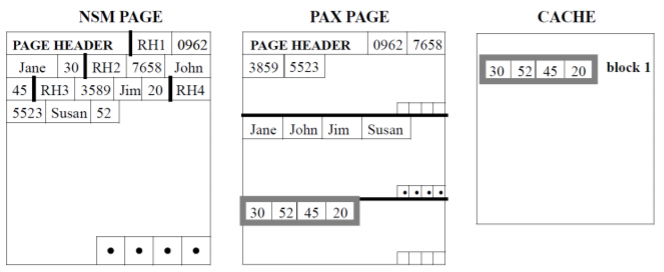
\includegraphics[scale=0.8]{images/2-pax.PNG}
	\caption{Row store (NSM) vs. PAX representation.}
	\label{fig:pax}
\end{figure}

\paragraph{Compression}
Not used to save space but rather to save bandwidth. There is a trade-off between the CPU cycles needed to (de)compress and the memory bandwidth (today: former wins, CPU much faster than memory). There is a possibility to process data in its compressed form. There are many different compression mechanisms and they depend on the data organization (dictionary, run length encoding, delta encoding, bitmaps, etc.).

\paragraph{Dictionary Compression}
Rather an encoding than actual compression. Build a dictionary that maps long entries to, for example, integers / small numbers when the data is loaded. This can be applied to any finite collection of names (e.g. countries, departments, etc.). The data can be easily processed in its encoded form. A hash function is one way to implement a dictionary encoding.

\paragraph{Frame of Reference}
Many attributes have value locality and can be represented as a delta over some base (e.g. 1007, 1017, 1090 represented as 1000, 7, 17 and 90). This allows for operations on compressed data. Can be combined with delta encoding for sorted lists of data (store difference to previous value rather than actual value).

\paragraph{Run Length Encoding}
If a value repeats, store it once and how many time it appears. Useful for attributes with low cardinality (e.g. departments). Often used in column store. For row store it is used for long strings with repeated characters. Compresses the data significantly but processing is more complex. The encoding is variable in size.

\paragraph{Bit-Vector Representation / Bitmap}
For every value that an attribute may take, construct the bitmap as follows: create array as long as number of tuples, if tuple i has value x for that attribute, position i in the bitmap x is set to 1. Bitmaps act as an index and can be used to process queries just by looking at it (selections, joins on an attribute, group by on attribute, etc.). Can be further compressed using run length encoding - but processing becomes more complex.





\subsection{Indexing}

An index is a data structure that improves the speed (sub-linear time) of data retrieval operations (random and sequential) on a database table at the cost of additional writes and storage space (as in B+ Trees) - or processing power (as in hashing) - to maintain the index data structure. It can be stored on either disk or RAM. An index can also be used to police database constraints when data is inserted / updated (i.e. unique, exclusion, primary / foreign key). A DB index is the same concept as an index at the end of a textbook indicating on which page(s) certain topics can be found.

Usually, when data is loaded into storage, it has no order = heap. The records are simply put into empty blocks and when a block is full, move to the next free block. The records of a table can therefore span over multiple physical data blocks residing on disk. Records are accessed by specifying the disk sector, disk row = block (usually 521 bytes) and block offset. An index is another way to logically represent data which has the advantage to make its retrieval more efficient.


\subsubsection{Hashing}

Hashing can be used to construct an index but also as a partitioning strategy when allocating data. A hash is not really an index but it is one way to implement an indexing functionality. A hash index is used to create physical addresses for records (usually using their primary key as input to the hash function).

\paragraph{Hash Function}
A function applied to some kind of arbitrary sized value (e.g. a single attribute value of a table) resulting in a fixed-size hash value. A hash value is usually much smaller than the original value. Different values might result in the same hash value since they are fixed in size (= collision).

There are many functions with strong properties but in a DB the function has to be computationally cheap (usually a modulo operation) since it is used very often.

\paragraph{Hash Table}
A structure that maps keys (usually primary key) to values. It uses a hash function to compute an index for an array of buckets / slots (in DB: bucket = typically a block) that contain the desired values. To look up a desired value, the key is hashed and the location of it is found with the resulting index. This only works for point queries.

Collisions do not happen with perfect hash functions but the table needs to be as big as the cardinality of the attributes (e.g. 4 byte keys = 4 GB table). But if the table is too small, we have too many collisions. Growing the hash table is an expensive operation. Choosing the perfect size is key.

\paragraph{Dealing with Collisions / Static Hashing}
Since a bucket in a DB is usually a block and not a single tuple, i.e. colliding values might simply belong to the same block, we have less "bad" collisions - this usually means that we ran into a block that is full and we to allocate a new one. Ways to deal with such collisions include:

\begin{itemize}
    \item \textbf{Closed Hashing / Chaining:} Add a block with free space to the linked list pointed to by a hash bucket. Not optimal because locating the desired tuple is now more complex (especially if the linked list is long). Improve efficiency by already adding free blocks to a linked list before collision even occurs.
    \item \textbf{Open Hashing:} Look for an empty slot in the hash table using some rule. Linear probing: simply add tuple to the block with index = index + 1. Cuckoo hashing: use several hash functions, if the first one leads to a collision use the next one and so on.
\end{itemize}

\paragraph{Growing the Hash Table / Dynamic Hashing}
This needs to be done when the hash table is completely full. A basic approach would be to create a new, larger hash table with more buckets (typically 2x) and rehash all the existing tuples. Very expensive and inefficient, lots of random accesses and cannot be done on disk (where hash indices are mostly used). Other approaches are often used in combination or in a nested manner (bucket directory pointing to another hash table pointing to actual data - helps with skew).

\textbf{Extendible Hashing:} Instead of having each hash value uniquely identify its own bucket, several hash values point to the same bucket and therefore the same block. If a block fills up, split it and move entries as needed. This increases the available space without significantly changing the hashing mechanism but it requires two page lookups (bucket directory and data block). To allow for more splitting (higher degree of sharing), the size of the table / bucket directory can be doubled by adding another bit to the matching value which increases the number of buckets = logical doubling. %TODO better?

\textbf{Linear Hashing:} A split pointer is used to indicate which bucket will be split in case of overflow (which is not necessarily the one that actually overflows - this one is simply chained) or other triggers (load factor, max. chain length, etc.). The entries targeted by the split bucket use a second hash function targeting the expanded range (mod n, mod 2n). After splitting, move the pointer to the next block. With this, the size of the hash table is gradually increased while redistributing the table (pointer hitting a chained block). The directory grows page by page instead of doubling. Once all buckets have been split, start anew. %TODO better


\subsubsection{B+ Tree Index}

B+ Trees are used to create an index by trading in space. No matter what is said, a DB always uses B+ Trees, never B-Trees. With a B+ Tree index, we always have to specify what we are indexing on (one or multiple attributes). An index sorts the specified attribute value(s) with each row including a pointer to the actual memory location of the block containing the respective record. Pointers can also point to another index and so on. A table can have multiple indexes logically sorting it in many different ways.

It is infeasible to directly sort the physical data (base table) since it can be highly dynamic and we might want to sort it on different (combinations of) attributes for different queries.

One of the best videos to watch is \href{https://www.youtube.com/watch?v=aZjYr87r1b8}{this one}. Explains why and what B-Trees are and how they relate to a DBMS.


\paragraph{Clustered Index / Primary Index}
A clustered index of a table defined on a certain (set of) attribute(s) (predicate) \textbf{physically} sorts the data according to the index when storing it on disk. The leaf nodes (see later) include the actual base table data (divided into blocks, not single rows!). There can only be one clustered index per table. When the clustered index is defined over a set of attributes, it is impossible to access it using a subset of these attributes.

A clustered index is typically created automatically when loading data into the DB using the primary key as the index attribute. Very efficient for data that is not updated frequently. When inserting new values, remaining free space on the blocks is filled and if a block is full, indirection is necessary (see previous sections).

\paragraph{Non-Clustered Index / Secondary Index}
An index defined over a certain (set of) attribute(s) (predicate) with leaf nodes containing pointers to the physical data stored on disk. The physical data may be stored as a simple heap or if a clustered index is present, a non-clustered index may point to the key values present in the clustered index (kinda like two seek operations). There can be multiple non-clustered on different predicates defined on the base table.

\paragraph{Index Key}
An index has to be defined over a certain predicate. It can either be a single attribute (e.g. primary key) or a combination of attributes. A composite key is compared lexicographically:

$$
(a1,b1) < (a2,b2) \Longleftrightarrow (a1 < b1) \lor (a1 = b2 \land a2 < b2)
$$



\paragraph{B-Tree}
Self-balancing tree that maintains sorted data and allows for searches, sequential access, insertions and deletions in logarithmic time. It requires linear space. It is a generalization of a binary tree since it allows for more than two children per node.

\begin{itemize}
    \item Order = $m$.
    \item Every node has at most $m$ children.
    \item Every non-leaf node except root has at least $\frac{m}{2}$ (round up) children.
    \item If it is not a leaf, the root has at least two children.
    \item A non-leaf node with $k$ children contains $k-1$ keys.
    \item All leaves appear in the same level.
\end{itemize}

If a B-Tree is used as an index, each node contains several pointers to data referenced by the keys present in the node (on top of the pointers to the child nodes).

%TODO good example

A B-Tree is constructed bottom up. Whenever a node is full, it is split and the parent node is updated to correctly reference its children.

\paragraph{B+ Tree}
Is a B-Tree where the data is at the leaves only (actual data or pointers to the data). The leaf nodes are organized as a linked list. Each key in the inner nodes is repeated accordingly in the leaves. The values in the same leaf node might point to different data blocks.

Indexes are referred by segments and they can use different block sizes (= nodes) than actual data blocks. Furthermore, an index can have its own memory buffer to avoid that something working on the index affects something working on the data.

%TODO good example


\paragraph{Non-Unique Values}
A B+ Tree index can be built on any attribute including those that are not unique. To differentiate duplicates, we can either repeat the key at the leaf nodes for every duplicate entry or store the key once and let it point to a linked list of all the matching entries. If the data is stored directly in the leaves, append the tuple ID to differentiate tuples the entries are referring to. %TODO what does this look like exactly, reading

\paragraph{Direct Lookup}
To find a single tuple, traverse the tree starting from the root. Within each node, use binary search to look for the correct entry. At the leaf node: return the corresponding pointer / position.

\paragraph{Range Lookup}
To find tuples that are in a particular range, start by finding the leaf node corresponding to the first value and then follow the linked list until we hit the second value.

\paragraph{Insertion}
Lookup the corresponding leaf. If there is space, insert. If there is no space, split leaf into two, insert item and insert new separator on parent node. If parent node is full, split it in two and insert separator in parent's parent node. Go all the way to the root if necessary. %TODO example

\paragraph{Deletion}
Lookup the corresponding leaf and remove entry. If the leaf is less than half order full, check a neighboring leaf. If it is more than half full, balance both. If it is half full, merge both. Update separator(s) in parent. %TODO example

\paragraph{Concurrent Access}
Use lock coupling to protect index from conflicting concurrent accesses. When accessing the index, first lock the root and the first level. Check where you have to go and only then release first lock on root. Lock second level and repeat up to the leaf level. %TODO lock on entire level or on one node of level? %TODO more, splitting p.29/30

%TODO index locking

\paragraph{Creating a B+ Tree Index}
A B+ Tree is created bottom up (leaves first):

\begin{itemize}
    \item Sort the data
    \item Fill blocks one after another (leave space if updates are anticipated else we have a clustered and compact tree)
    \item Remember largest value in each block %TODO or left/right bias
    \item Create inner nodes by using largest value in each block as separator
    \item Iterate upwards to the next level until there is only a single block (root)
\end{itemize}

\paragraph{Optimizations}
\begin{itemize}
    \item \textbf{Reverse Index:} If the indexed attribute is a sequence and new items are constantly produced, insert items by reversing them so that they are more likely to go to different blocks. This protects from concurrent updates fighting to insert on the same block.
    \item \textbf{More Efficient Keys:} Replace keys in inner nodes with shorter separators that have the same effect or factor the children's common prefix. %TODO insert images
    \item \textbf{Ignore Rules:} Don't merge nodes when they do not have enough data - delaying a merge can minimize changes. Periodically rebuild the tree instead. Also: using variable length keys might improve efficiency, but it is more complex. %TODO
    \item Wide / shallow trees are good for slow storage devices (large nodes, potentially over several sequential blocks) and deep trees are good for fast storage devices (small nodes, potentially several for one block).
\end{itemize} %TODO See paper


\subsubsection{Other Indexing Techniques}

\paragraph{Query Selectivity}
Selectivity refers to the number of tuples returned by the query. A highly selective query returns very few tuples as a result (vs. low selectivity). The indices discussed above work well for queries with high selectivity.

For low selectivity, a table scan might be a good index. %TODO?

\paragraph{Bitmaps}
Simple predicate selections can be very efficient using bitmaps by intersecting them for every queried column. Since bitmaps are usually sparse, they can be compressed pretty well (with run length encoding) and they are often used for large tables in OLAP - faster than other indices for low selectivity queries. Especially useful for data types where comparison is expensive. %TODO example

\paragraph{Materialized Aggregates}
For groups of data that don't change very often, one can compute and store some basic statistics = aggregates (sum, avg, count, min, max, etc.). These can be used as small indices to check whether the data needed is within that group. They can also be used to compute aggregates over the whole table without having to read all of it.

\paragraph{Specialized Indexes}
\begin{itemize}
    \item \textbf{Trie / Prefix Tree:} Tree data structure used to store a dynamic set where the keys are usually strings. The value of a key is distributed across the nodes. See example in Figure \ref{fig:trie}.
    \item \textbf{Patricia Tree:} A type of radix tree (= space-optimized Trie).
    \item Inverted indexes, R-Trees, Grid File, etc.
\end{itemize}

\begin{figure}[h]
	\centering
	\includegraphics[scale=0.4]{images/2-trie.png}
	\caption{Trie example.}
	\label{fig:trie}
\end{figure}





\subsection{Access Methods in Context}

Alternative designs for representing data in memory.

\paragraph{Denormalized Tables}
Usually, normal forms (rules) are used to eliminate redundancy in a DB schema by forcing table splits until each different table represents a distinct concept. This saves space but it is common that the split tables will be joined again in almost every query. Denormalized tables allow for more than one table to be stored in the same blocks by clustering the tables into the same segment (blocks are indexed by the common attribute) = materialized join. This reduces I/O and saves space but updates are more expensive. E.g. Clustered Tables in Oracle, see Figure \ref{fig:cluster}.

\begin{figure}[h]
	\centering
	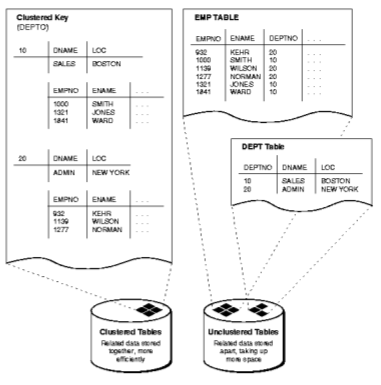
\includegraphics[scale=0.8]{images/2-cluster.PNG}
	\caption{Oracle: Clustered Tables.}
	\label{fig:cluster}
\end{figure}

\paragraph{Log Structured Databases}
Instead of storing tuples and modifying them as needed, only store a record of how the data is modified (a log). With this, inserts record the entire tuple, deletes indicate that a tuple is invalidated and updates record modified tuples (no in-place updates). New log entries are simply appended at the end of the log file (much faster than random access). Mainly used for in-memory OLTP (minimizes cost for making data persistent) and cloud storage (file storage is typically append only). Not useful for heavy OLAP. To optimize this concept, the log file is periodically compacted (remove history by adding only one entry for each tuple - all operations are applied) and the tuples and their modifications are indexed. %TODO more?

\paragraph{No Indexes}
Snowflake uses micro-partitions instead of indices (see previous section) and MonetDB (column store) uses database cracking: the index is built incrementally while the data is being processed on a column-wise basis. Initial queries are expensive but later cost us amortized as (some) work has already been done. See example in Figure \ref{fig:crack}. %TODO more?

\begin{figure}[h]
	\centering
	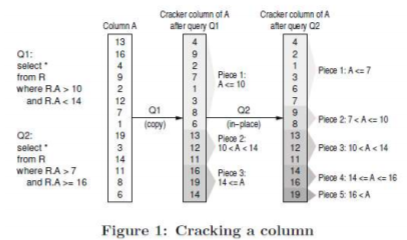
\includegraphics[scale=0.8]{images/2-crack.PNG}
	\caption{Database cracking example.}
	\label{fig:crack}
\end{figure}





\subsection{Reading Assignments}


\subsubsection{Modern B-Tree Techniques}


\paragraph{B-Tree vs. Hash Index}
Argument for hash index: single I/O per lookup and CPU efficient due to efficient comparisons and address calculations. But:
\begin{itemize}
    \item I/O: if branch nodes are in buffer, B-Tree is also single I/O.
    \item CPU: Just use hash values as keys (or other efficient keys).
    \item Straightforward space management.
    \item Multi-field indexes and nonuniform distributions of key values.
    \item Efficient index creation. Online creation possible.
    \item Support for ordered scans and range predicates.
    \item etc.
\end{itemize}

\paragraph{Key Normalization}
To reduce the cost of key comparisons, transform keys into binary strings s.t. simple binary comparisons suffice to sort the records during index creation and to guide a search. Key sequence for sort order of original key and binary string have to be the same and all comparisons equivalent. Binary strings may also encode multiple columns and additional information. Also allows for easy compression. %TODO example





\subsubsection{The Design and Implementation of Modern Column-Oriented Database Systems}

\paragraph{Compression Ratio}
CS has an improved compression ratio compared to RS since each column can be compressed in a different way. Since many compression ratios compress data in a non-fixed way, using virtual IDs to identify single items in a column becomes more complex.

\paragraph{Late Materialization}
Delay the joining of columns into wider tuples. Possible in CS since it allows for processing data in a columnar format.

\paragraph{C-Store}
\begin{itemize}
    \item Data on disk is represented as a set of column files with each file containing data from a single column - compressed in a column-specific manner and sorted on the column attribute. = Read Optimized Store (ROS)
    \item Newly loaded data is stored in Write Optimized Store (WOS) - uncompressed and not vertically partitioned.
    \item Both ROS and WOS are accessed when processing a query.
    \item Data is periodically moved from WOS to ROS by a tuple mover (sort, compress, divide and write to disk).
    \item A column may be stored several times in different sort orders (to process frequent queries efficiently).
    \item Projection = group of columns sorted on same attribute. There is at least one containing all columns and it can be used to answer any query.
    \item Column-specific compression depends on if column is sorted, its data type and the number of its distinct values.
    \item No secondary indexes on tables.
    \item Sparse indexes: indexing into sorted projections. It stores the first value contained on each physical page of a column.
    \item No-overwrite storage representation: updates are deletes followed by inserts. Deletes are processed by storing a delete column recording the time every tuple was deleted (if).
    \item Queries are run as of a specific time to filter out deleted tuples. This allows time travel.
    \item DB modification uses two-phase locking.
    \item Based on a shared-nothing architecture. Projections are horizontally partitioned.
\end{itemize}

\paragraph{MonetDB}
\begin{itemize}
    \item Data is stored column-wise both in memory and on disk (uncompressed on disk). Exploits bulk processing and late materialization. Profits from SIMD instructions. Push-based operators.
    \item No buffer pool, only memory-mapped files. %TODO Virtual mem?
    \item Column-at-a-time algebra.
    \item %TODO BAT Algebra stuff...
    \item Intermediate results are fully materialized. See materialized execution model.
    \item
    \item Processing algorithms, that minimize CPU cache misses rather than IOs
    \item Indexing, which is not a DBA task but happens as a by-product of query execution, i.e., database cracking
    \item Query optimization, which is done at run-time, during query incremental execution
    \item Transaction management, which is implemented using explicit additional tables and algebraic operations, so read-only workloads can omit these and avoid all transaction overhead
\end{itemize}

\paragraph{VectorWise}
\begin{itemize}
    \item Balance between full materialization of intermediate results as in MonetDB and the tuple-at-a-time iterator model. See vectorized execution model.
    \item Using Positional Delta Trees for updates.
    \item If there is an arithmetic operation only for small number of values selected in an array, VectorWise can compute this operation for all the array, even though it is not necessary.
    \item VectorWise tunes the vector size such that all vectors for evaluating a query together fit in the CPU cache.
    \item 
\end{itemize}

Loop pipelining → Mapping loops into optimized pipeline executions, Array blocking → Grouping subsets of an array to increase cache locality, Strength reduction → Replacing an operation with an equivalent less costly operation

The typical size of each vector in vectorized execution does not fit the L2 cache.

RLE: (value, start position, runLength) triples

Late materialization can benefit from selection and aggregation operators.


NSM: record header, DSM: record ID, columns, PAX: mini pages






\subsubsection{Data Page Layouts for Relational Databases on Deep Memory Hierarchies}


%TODO PAX wiki



\subsubsection{A Hybrid Page Layout Integrating PAX and NSM}

See Figure \ref{fig:pax} for difference between NSM and PAX.

\paragraph{PAX}
Each page is partitioned into n minipages (degree of relation). Values of the first attribute are stored in first minipage and so on. Page header contains pointers to beginning of each minipage. Fixed-length attributes are stored in F-minipages with a presence bit vector at the end for each entry - it indicates null values. Variable-length attributes are stored in V-minipages with pointers pointing to the end of each slot.

\paragraph{PAX Disadvantage}
Complexity of free space management withing a page for records with one or more variable-sized fields.

\paragraph{Hybrid Page Layout (HPL)}
Combines NSM and PAX. From NSM: two variable-sized allocation spaces growing towards each other. From PAX: cache efficiency during large scans.

\paragraph{Simple Segments}
Simplest HPL variant. Allocation space for fixed sized fields grows from one end, allocation space for variable sized fields from the other. Offsets for V-fields are their own fixed sized fields.


Set of records in the F fields is divided into segments. Number of records per segment = number of bytes per cache line. With 13 total bytes of F field values, we have 13 cache lines per segment.

%TODO






\subsection{Exercises}

\subsubsection{Column-Store}

\subsubsection{Page Layouts and Indexing}

\subsubsection{Indexing}
